
\section{Resultados}

\lettrine{P}{rimeiramente}, foram realizadas simulações para o caso em que a probabilidade p
de envenenamento é muito baixa. No caso extremo, essa probabilidade é 0 e o
sistema se comporta de acordo com a equação \ref{Equation-027-Decaimento}, para
sistemas sem envenenamento. Mas como mostrado pela figura
\ref{Figure-052-Resultado}, essa equação descreve bem sistemas com p pequenos.
Nesses sistemas, em que $\sigma_0 >> p*\theta_0$, é possível perceber pela
figura que a quantidade de reagentes decaem em uma lei de potência e tendem a
acabar com o passar do tempo. Esse comportamento é esperado já que o
envenenamento ocorre com pouca frequência no sistema com esse tipo de regime,
então a chance dos regentes reagirem e saírem do sistema é grande. Por isso, o
sistema tende a perder poucos catalisadores e perder todos os reagentes.

{
	\captionsetup{type=figure}
	\hfill \break
	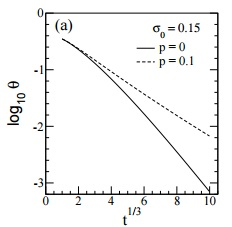
\includegraphics[width=\columnwidth]{./figures/052-Resultado.jpg}
	\captionof{figure}{Comportamento dos reagentes com o tempo para regimes em que
		os regentes tendem a se extinguir}
	\label{Figure-052-Resultado}
}

Posteriormente, foram realizadas simulações para o caso em que o sistema possui
probabilidade de envenenamento p alta e concentração inicial de reagentes
$\theta_0$ também alta ao passo que a concentração inicial de catalisadores
$\sigma_0$ se manteve constante. Sistemas com esse regime apresentam um
decaimento de reagentes muito grande no início, já que a concentração deles
é grande, mas com o passar do tempo esse decaimento vai ocorrendo de forma
cada vez mais lenta até que não haja mais nenhum decaimento, como pode ser
observado na figura \ref{Figure-053-Resultado}. Isso ocorre porque a chance de
ocorrer envenenamento é grande, o que faz com que o decaimento do número de
reagentes também seja grande e, no fim, todos os catalisadores são desativados e
os reagentes restantes permanecem no sistema.

{ \centering
	\captionsetup{type=figure}
	\hfill \break
	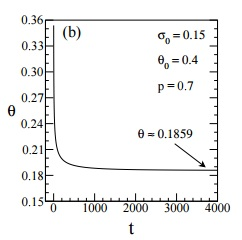
\includegraphics[width=\columnwidth]{./figures/053-Resultado.jpg}
	\captionof{figure}{Comportamento dos reagentes com o tempo para regimes em que
	 	os catalisadores tendem a se extinguir}
	\label{Figure-053-Resultado}
}

Também foram simulados sistemas de reação-difusão com envenenamento na
criticalidade, ou seja, sistemas nos quais $\sigma_0 = p*\theta_0$. Como
esperado, percebe-se na figura \ref{Figure-051-Resultado} um decaimento em lei
de potência do número de reagentes no tempo para esses sistemas e, além disso,
as curvas em uma escala log-log apresentam uma reta com inclinação de,
aproximadamente, $-1/4$, como prevê a equação REFERENCIAR!!.

{ \centering
	\captionsetup{type=figure}
	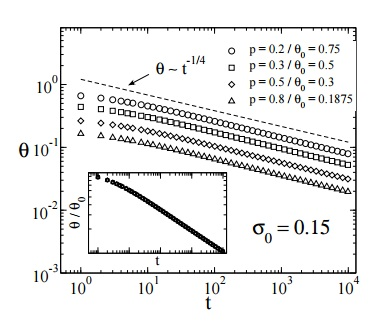
\includegraphics[width=\columnwidth]{./figures/051-Resultado.jpg}
	\captionof{figure}{Comportamento dos reagentes no tempo em um sistema de
		reação-difusão na criticalidade. No inset observa-se todas as curvas
		colapsadas}
	\label{Figure-051-Resultado}
}

As simulações já apresentadas descrevem sistemas com envenenamento longe da
criticalidade e exatamente na criticalidade. As últimas simulações descrevem
sistemas próximos da criticalidade, com regimes em que os reagentes tendem a
acabar ($\sigma_0 > p*\theta_0$). A figura \ref{Figure-054-Resultado} descreve
esses sistemas próximos da criticalidade e, como pode-se perceber, no início os
reagentes decaem de acordo com a lei de potência prevista para sistemas na
criticalidade (o início dos sistemas no primeiro gráfico apresenta comportamento
semelhante ao observado na figura \ref{Figure-051-Resultado}), mas em tempos
longos, o sistema se comporta como aquele da figura \ref{Figure-052-Resultado}.
A semelhança pode ser notada comparando o segundo gráfico da figura
\ref{Figure-054-Resultado} com a figura \ref{Figure-052-Resultado}.

{ \centering
	\captionsetup{type=figure}
	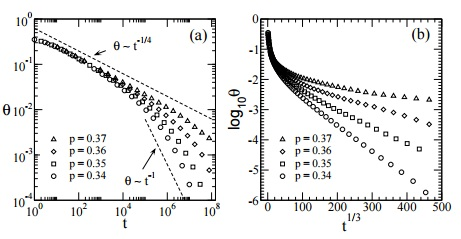
\includegraphics[width=\columnwidth]{./figures/054-Resultado.jpg}
	\captionof{figure}{Comportamento dos reagentes no tempo em sistemas de
		reação-difusão próximos da criticalidade}
	\label{Figure-054-Resultado}
}
